\section{Retas e Planos}

\subsection*{Equação Paramétrica da Reta}


\begin{frame}[label=retas]{Equação Paramétrica de uma Reta}


Sabemos que uma reta $r$ pode ser inteiramente descrita por {\color{blue} equação vetorial paramétrica}
\[P={\color{red}A}+t{\color{blue}\vec{v}},\ t\in \R.\]
	\begin{center}
		\begin{tikzpicture}
		\tikzset{>=latex}
		\draw[thick] (-1,-1) -- (2,2);
		\node[left] at (2,2) {r};
		\draw[fill=red] (0,0) circle [radius=1.5pt];
		\node[above left] at (0,0) {$\textcolor{red}{A}$};
		\draw[thick, blue,->] (2,0) -- (0.7+2,0.7);
		\node[blue, right] at (0.7+2,0.7) {$\vec{v}$};
		\onslide<2->{
		\draw[fill=black] (1.5,1.5) circle [radius=1.5pt];
		\node[above left] at (1.5,1.5) {$P$};}
	
	\onslide<3->{
\draw[thick, blue,->] (0,0) -- (1.5,1.5);	
  }
		\end{tikzpicture}
	\end{center}
onde ${\color{red} A}$ é um ponto fixado de $r$ e  ${\color{blue}\vec{v}}$ é um vetor diretor desta reta.
	
\end{frame}

\begin{frame}[label=retas]{Em coordenadas}
Se	$P=(x,y)$, $\textcolor{red}{A=(x_0,y_0)}$ e $\textcolor{blue}{\vt{v}=(a,b)}$
\[	r: \left\{\begin{array}{l}
	x=\textcolor{red}{x_0}+\textcolor{blue}{a}t\\
	y=\textcolor{red}{y_0}+\textcolor{blue}{b}t,\  t\in \R.
	\end{array}\right.\]

Se 	$P=(x,y,z)$, $\textcolor{red}{A=(x_0,y_0,z_0)}$ e $\textcolor{blue}{\vt{v}=(a,b,c)}$
		\[r:	\left\{\begin{array}{l}
		x=\textcolor{red}{x_0}+\textcolor{blue}{a}t\\
		y=\textcolor{red}{y_0}+\textcolor{blue}{b}t\\
		z=\textcolor{red}{z_0}+\textcolor{blue}{c}t,\  t\in \R.
		\end{array}\right.\]
		Estas equações são chamadas simplesmente de \dest{equações paramétricas  da reta} $r$.


\end{frame}


\begin{frame}[label=retas]
	\frametitle{ }
	%\begin{scriptsize}
	{\begin{exe}\label{exer4} \noindent
			
			\begin{enumerate}[a]
			\item Determinar  as equações paramétricas da reta $r$ que passa pelos
				pontos $A = (1, 2, -2)$ e $B = (-1, 4, 2)$.

	\item\label{ex6} Sejam $A=(0,1,8), B=(-3,0,9)$ e $r: X=(1,2,0)+t(1,1,-3)$. Determine o ponto $C$ de $r$ tal que $A,B$ e $C$ sejam vértices de um triângulo retângulo com ângulo reto no vértice $A$.
			\end{enumerate}
	\end{exe}}

\end{frame}
%%%%%%%%%%%%%%%%%%%%%%%%%%%%%%%%%%%%%%%%%%%%%%%%%%%%%%%%%%%%%

\subsection*{Equação Cartesiana do Plano no Espaço}

\begin{frame}[label=planos]{Equação Cartesiana do Plano no Espaço}
Sejam  ${\color{red}A=(x_0,y_0,z_0)}$  um ponto de um plano em $\R^3$, $\textcolor{blue}{\vt{n}=(a,b,c)}\perp \pi$, então os pontos e  $P=(x,y,z)$do plano devem satisfazer a seguinte \dt{equação cartesiana}
\[{\color{blue}a}x+{\color{blue}b}y+{\color{blue}c}z+{\color{red}d}=0\]
\begin{center}
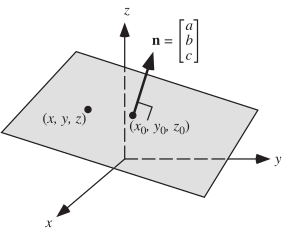
\includegraphics[scale=0.8]{figuras/normal-vector.png}
\end{center}
\end{frame}

\begin{frame}
\begin{exe}
\begin{enumerate}


\item Determine a equação do plano que passa por $A=(1,3,2)$, $B=(3,-1,6)$ e $C=(5,2,0)$. 

\item Determine o ponto da reta 
\[r: \begin{cases} x=2+3t,\\ y=-4,\\ z=5+t, \ \ t\in \R. \end{cases}
\]
que intercepta o plano $4x+5y-2z=18$.


\item Determine a equação do plano que passa pelo ponto $A=(1,0,1)$ e é perpendicular à reta $r: X=(-1,1,2)+t(-1,2,1),\ t\in \R$.
 
\end{enumerate}

\end{exe}

\end{frame}



%%%%%%%%%%%%%%%%%%%%%%%%%%%%%%%%%%%%%%%%%%%%%%%%%%%%%%%%%%%%%

\begin{frame}[label=planos]
	\begin{casa}
\begin{enumerate}
\item Determine uma equação para o plano que passa pelos pontos $A=(0,1,1)$, $B=(1,0,1)$ e $C=(1,1,0)$.

\item Determine as equações paramétricas da reta dada pela interseção dos planos
$x+y+z=1$ e $x-2y+3z=1$.

\item Determine as equações paramétricas da reta que passa pelo ponto $(1,0,6)$ e é perpendicular ao plano $x+3y+z=5$.
\end{enumerate}
	\end{casa}
\end{frame}